\documentclass[12pt]{beamer}
\usepackage{../Estilos/BeamerMAF}
\usepackage{../Estilos/ColoresLatex}
%Sección para el tema de beamer, con el theme, usercolortheme y sección de footers
\usetheme{Frankfurt}
\usecolortheme{beaver}
%\useoutertheme{default}
\setbeamercovered{invisible}
% or whatever (possibly just delete it)
\setbeamertemplate{section in toc}[sections numbered]
\setbeamertemplate{subsection in toc}[subsections numbered]
\setbeamertemplate{subsection in toc}{\leavevmode\leftskip=3.2em\rlap{\hskip-2em\inserttocsectionnumber.\inserttocsubsectionnumber}\inserttocsubsection\par}
% \setbeamercolor{section in toc}{fg=blue}
% \setbeamercolor{subsection in toc}{fg=blue}
% \setbeamercolor{frametitle}{fg=blue}
\setbeamertemplate{caption}[numbered]

\setbeamertemplate{footline}
\beamertemplatenavigationsymbolsempty
\setbeamertemplate{headline}{}


\makeatletter
% \setbeamercolor{section in foot}{bg=gray!30, fg=black!90!orange}
% \setbeamercolor{subsection in foot}{bg=blue!30!yellow, fg=red}
% \setbeamercolor{date in foot}{bg=black, fg=white}
\setbeamertemplate{footline}
{
  \leavevmode%
  \hbox{%
  \begin{beamercolorbox}[wd=.333333\paperwidth,ht=2.25ex,dp=1ex,center]{section in foot}%
    \usebeamerfont{section in foot} \insertsection
  \end{beamercolorbox}%
  \begin{beamercolorbox}[wd=.333333\paperwidth,ht=2.25ex,dp=1ex,center]{subsection in foot}%
    \usebeamerfont{subsection in foot}  \insertsubsection
  \end{beamercolorbox}%
  \begin{beamercolorbox}[wd=.333333\paperwidth,ht=2.25ex,dp=1ex,right]{date in head/foot}%
    \usebeamerfont{date in head/foot} \insertshortdate{} \hspace*{2em}
    \insertframenumber{} / \inserttotalframenumber \hspace*{2ex} 
  \end{beamercolorbox}}%
  \vskip0pt%
}







\setbeamercolor{section in foot}{bg=deepcarmine, fg=white}
\setbeamercolor{subsection in foot}{bg=flame, fg=white}
\setbeamercolor{date in foot}{bg=blue, fg=white}

\makeatletter
\setbeamertemplate{footline}
{
\leavevmode%
\hbox{%
\begin{beamercolorbox}[wd=.333333\paperwidth,ht=2.25ex,dp=1ex,center]{section in foot}%
  \usebeamerfont{section in foot} \insertsection
\end{beamercolorbox}%
\begin{beamercolorbox}[wd=.333333\paperwidth,ht=2.25ex,dp=1ex,center]{subsection in foot}%
  \usebeamerfont{subsection in foot}  \insertsubsection
\end{beamercolorbox}%
\begin{beamercolorbox}[wd=.333333\paperwidth,ht=2.25ex,dp=1ex,right]{date in head/foot}%
  \usebeamerfont{date in head/foot} \insertshortdate{} \hspace*{1.5em}
  \insertframenumber{} / \inserttotalframenumber \hspace*{2ex} 
\end{beamercolorbox}}%
\vskip0pt%
}
\makeatother
\usefonttheme{serif}
\setbeamercolor{frametitle}{bg=lavenderblue}
\resetcounteronoverlays{saveenumi}

\date{}

\title{\large{Tema 5 - Funciones asociadas de Legendre}}
\subtitle{Funciones Especiales }
\author{M. en C. Gustavo Contreras Mayén}

\begin{document}
\maketitle
\fontsize{14}{14}\selectfont
\spanishdecimal{.}

\section*{Contenido}
\frame[allowframebreaks]{\tableofcontents[currentsection, hideallsubsections]}

%Referencia Riley. 18.2 Funciones asociadas de Legendre

\section{Funciones asociadas de Legendre.}
\frame{\tableofcontents[currentsection, hideothersubsections]}
\subsection{Definición}

\begin{frame}
\frametitle{La ecuación diferencial}
La ecuación asociada de Legendre tiene la forma:
\pause
\begin{equation}
(1 - x^{2}) \sderivada{y} - 2 \, x \, \pderivada{y} + \left[ \ell (\ell + 1) - \dfrac{m^{2}}{1 - x^{2}} \right] \, y = 0
\label{eq:ecuacion_18_28}
\end{equation}
\pause
que tiene tres puntos singulares en $x = -1, 1, \infty$, se reduce a la ecuación de Legendre (\ref{eq:ecuacion_18_01}) cuando $m = 0$.
\end{frame}
\begin{frame}
\frametitle{Naturaleza de la ED}
Se presenta en problemas de la física que involucran el operador $\nabla^{2}$, cuando se expresa en coordenadas esféricas.
\\
\bigskip
\pause
En esos casos, $- \ell \leq m \leq \ell$ y $m$ está restringida a valores enteros.
\end{frame}
\begin{frame}
\frametitle{Naturaleza de la ED}
Como en el caso de la ecuación de Legendre, la variable $x$ es el coseno del ángulo polar en coordenadas esféricas, por tanto $-1 \leq x \leq 1$.
\\
\bigskip
\pause
Cualquier solución de la ecuación \ref{eq:ecuacion_18_28}) es llamada la \textocolor{ao}{función asociada de Legendre}.
\end{frame}
\begin{frame}
\frametitle{Estudiando la ED}
El punto $x = 0$ es un punto ordinario, y del cual se pueden obtener soluciones en series de la forma:
\pause
\begin{align*}
y (x) = \nsum_{n=0} a_{n} \, x^{n}
\end{align*}
de la misma manera que se hizo para la ecuación de Legendre.
\end{frame}
\begin{frame}
\frametitle{Estudiando la ED}
En este caso, debemos de notar que si $u (x)$ es solución de la ecuación de Legendre, entonces:
\pause
\begin{equation}
y (x) = (1 -x^{2})^{\abs{m}/ 2} \dv[\abs{m}]{u}{x}
\label{eq:ecuacion_18_29}
\end{equation}
es solución a la ecuación asociada.
\end{frame}
\begin{frame}
\frametitle{Soluciones independientes}
De las dos soluciones en series linealmente independientes de la ecuación de Legendre dada por:
\pause
\begin{align*}
y_{1} (x) &= 1 - \ell (\ell + 1) \dfrac{x^{2}}{2!} + \\[0.5em]
&+ (\ell - 2)\; \ell \; (\ell + 1)\;(\ell + 3) \dfrac{x^{4}}{4!} - \ldots
\end{align*}
\end{frame}
\begin{frame}
\frametitle{Soluciones independientes}
Y por:
\pause
\begin{align*}
y_{2} (x) &= x - (\ell - 1)(\ell + 2) \dfrac{x^{3}}{3!} + \\[0.5em]
&+ (\ell - 3) (\ell - 1)(\ell + 2)(\ell + 4) \dfrac{x^{5}}{5!} - \ldots
\end{align*}
que ahora denotamos por $u_{1} (x)$ y $u_{2}(x)$.
\end{frame}
\begin{frame}
\frametitle{Soluciones independientes}
Podemos obtener dos soluciones en series linealmente independientes, $y_{1} (x)$ y $y_{2} (x)$, a la ecuación asociada mediante el uso de (\ref{eq:ecuacion_18_29}). 
\end{frame}
\begin{frame}
\frametitle{Soluciones independientes}
A partir de la discusión general de la convergencia de la series de potencias, vemos que tanto $y_{1} (x)$ como $y_{2} (x)$ también convergen para $\abs{x} < 1$.
\end{frame}
\begin{frame}
\frametitle{Solución general}
Por lo tanto la solución general de la ecuación(\ref{eq:ecuacion_18_28}) en este rango está dada por:
\pause
\begin{align*}
y(x) = c_{1} \, y_{1} (x) + c_{2} \, y_{2} (x)
\end{align*}
\end{frame}

\subsection{Asociadas de Legendre para enteros $\ell$}

\begin{frame}
\frametitle{Valores enteros}
Si $\ell$ y $m$ son ambos enteros, como suele encontrarse en varios problemas de la física, \pause entonces la solución general de la ecuación (\ref{eq:ecuacion_18_28}) se expresa por:
\pause
\begin{equation}
y (x) = c_{1} \, P_{\ell}^{m} (x) + c_{2} \, Q_{\ell}^{m} (x)
\label{eq:ecuacion_18_31}
\end{equation}
\pause
donde $P_{\ell}^{m} (x)$ y $Q_{\ell}^{m} (x)$ son las \textocolor{carmine}{funciones asociadas de Legendre de primera y segunda clase}, respectivamente.
\end{frame}
\begin{frame}
\frametitle{Valores negativos}    
Para valores no negativos de $m$, esas funciones están relacionadas a las funciones de Legendre para enteros $\ell$ mediante:
\pause
\begin{eqnarray}
\begin{aligned}
P_{\ell}^{m} (x) = (1 - x^{2})^{m/2} \, \dv[m]{P_{\ell}}{x} \\[1em] \pause
Q_{\ell}^{m} (x) = (1 - x^{2})^{m/2} \, \dv[m]{Q_{\ell}}{x}
\end{aligned}
\label{eq:ecuacion_18_32}
\end{eqnarray}
\end{frame}
\begin{frame}
\frametitle{Relación entre las funciones}
Vemos inmediatamente que, en caso necesario, las funciones asociadas de Legendre se reducen a las funciones ordinarias de Legendre cuando $m = 0$.
\end{frame}
\begin{frame}
\frametitle{Relación entre las funciones}
Dado que $m^{2}$ aparece en la ecuación asociada de Legendre (\ref{eq:ecuacion_18_28}), las funciones asociadas de Legendre para los valores negativos $m$ debe ser proporcional a la función correspondiente para valores no negativos $m$. 
\end{frame}
\begin{frame}
\frametitle{Relación entre las funciones}
La constante de proporcionalidad es una cuestión de convención.
\\
\bigskip
\pause
Para el $P_{\ell}^{m} (x) $, es habitual considerar la definición (\ref{eq:ecuacion_18_32}) como válida también para los valores negativos $m$.
\end{frame}
\begin{frame}
\frametitle{Relación entre las funciones}
Aunque la diferenciación de un número negativo no está definida, cuando $P_{\ell} (x)$ se expresa en términos de la fórmula de Rodrigues:
\pause
\begin{align*}
P_{\ell} (x) = \dfrac{1}{2^{\ell} \; \ell !} \, \dv[\ell]{x}  (x^{2} - 1)^{\ell}    
\end{align*}
este problema no se presenta para $\ell \leq m \leq \ell$. 
\end{frame}
\begin{frame}
\frametitle{Relación entre las funciones}
En este caso:
\pause
\begin{equation}
P_{\ell}^{-m} (x) = (-1)^{m} \, \dfrac{(\ell - m)!}{(\ell + m)!} \, P_{\ell}^{m} (x)
\label{eq:ecuacion_18_33}
\end{equation}
Ya que $P_{\ell}(x)$ es un polinomio de orden $\ell$, tenemos que $P_{\ell}^{m}(x) = 0$ para $\abs{m} > \ell$.
\end{frame}
\begin{frame}
\frametitle{Relación entre las funciones}
De esta definición, queda claro que $P_{\ell}^{m} (x)$ es también un polinomio de orden $\ell$ si $m$ es par, ya que contiene el factor $(1-x^{2})$ a una potencial fraccionaria si $m$ es impar.
\\
\bigskip
\pause
En cualquier caso $P_{\ell}^{m}(x)$ es regular en $x = \pm 1$.
\end{frame}
\begin{frame}
\frametitle{Funciones asociadas}
Las primeras funciones asociadas de Legendre de primera clase, se construyen fácilmente y están dadas por (se omiten los casos $m = 0$):
\end{frame}
\begin{frame}
\frametitle{Funciones asociadas}
\begin{eqnarray*}
\begin{aligned}
P_{1}^{1} (x) &= (1-x^{2})^{1/2} \\ \pause
P_{2}^{1} (x) &= 3x (1-x^{2})^{1/2}  \\ \pause
P_{2}^{2} (x) &= 3(1-x^{2})  \\ \pause
P_{3}^{1} (x) &= \frac{3}{2}(5x^{2}-1)(1-x^{2})^{1/2} \\ \pause
P_{3}^{2} (x) &= 15x (1-x^{2}) \\ \pause
P_{3}^{3} (x) &= 15 (1-x^{2})^{3/2} 
\end{aligned}
\end{eqnarray*}
\end{frame}
\begin{frame}[plain]
\begin{figure}
    \centering
    \includegraphics[scale=0.7]{Imagenes/plot_Asociados_Legendre_01.pdf}
\end{figure}
\end{frame}
\begin{frame}[plain]
\begin{figure}
    \centering
    \includegraphics[scale=0.7]{Imagenes/plot_Asociados_Legendre_02.pdf}
\end{figure}
\end{frame}
\begin{frame}[plain]
\begin{figure}
    \centering
    \includegraphics[scale=0.7]{Imagenes/plot_Asociados_Legendre_03.pdf}
\end{figure}
\end{frame}
\begin{frame}[plain]
\begin{figure}
    \centering
    \includegraphics[scale=0.7]{Imagenes/plot_Asociados_Legendre_04.pdf}
\end{figure}
\end{frame}
\begin{frame}
\frametitle{Singularidad en la función}
Debemos de mencionar que las funciones asociadas de Legendre de segunda clase $Q_{\ell}^{m} (x)$ como las $Q_{\ell}(x)$ son singulares en $x= \pm 1$.
\end{frame}

\subsection{Propiedades de \texorpdfstring{$P_{\ell}^{m}$}{P l m}}

\begin{frame}
\frametitle{Uso de un ángulo}
Cuando encontramos en problemas físicos, la variable $x$ de la ecuación asociada de Legendre (como en la ecuación ordinaria Legendre) es generalmente el coseno del ángulo polar $\theta$ en coordenadas polares esféricas.
\end{frame}
\begin{frame}
\frametitle{Uso de un ángulo}
Entonces queremos que la solución $y (x)$ sea regular en $x = \pm 1$ (correspondiente a $\theta = 0$ o $\theta = \pi$).
\end{frame}
\begin{frame}
\frametitle{Solución regular}
Para que esto ocurra, \pause se requiere que $\ell$ sea un número entero y que el coeficiente $c_{2}$ de la función $Q_{\ell}^{m} (x)$ en la ecuación (\ref{eq:ecuacion_18_31}) sea cero.
\end{frame}
\begin{frame}
\frametitle{Solución regular}
Dado que $Q_{\ell}^{m}(x)$ es singular en $x = \pm 1$, \pause con el resultado de que la solución general son múltiplos de las funciones asociadas de Legendre de primera clase $P_{\ell}^{m}(x)$.
\end{frame}

\subsection{Ortogonalidad mutua}

\begin{frame}
\frametitle{Ecuación autoadjunta}
Ya se mencionó anteriormente que la ecuación asociada de Legendre es del tipo Sturm-Liouville con:
\pause
\begin{eqnarray*}
\begin{aligned}
p &= 1 - x^{2} \\ \pause
q &= - \dfrac{m^{2}}{(1 - x^{2})} \\ \pause
\lambda &= \ell (\ell + 1) \\ \pause
w &= 1
\end{aligned}
\end{eqnarray*}
siendo su intervalo natural en $[-1,1]$.
\end{frame}
\begin{frame}
\frametitle{De la ortogonalidad}
Dado que las funciones asociadas de Legendre $P_{\ell}^{m} (x)$ son regulares en los extremos $x = \pm 1$, entonces deben de ser mutuamente ortogonales en este intervalo para un valor fijo de $m$.
\end{frame}
\begin{frame}
\frametitle{De la ortogonalidad}
Es decir:
\pause
\begin{equation}
\scaleint{6ex}_{-1}^{1} P_{\ell}^{m} (x) \, P_{k}^{m} (x) \dd{x} = 0, \hspace{1cm} \text{ si } \ell \neq k
\label{eq:ecuacion_18_36}
\end{equation}
Nótese que el valor de $m$ debe de ser el mismo en ambas funciones asociadas de Legendre para que la expresión sea válida.
\end{frame}
\begin{frame}
\frametitle{De la ortogonalidad}
La condición de normalización cuando $\ell = k$ se obtiene de la fórmula de Rodrigues:
\pause
\begin{equation}
\begin{aligned}[b]
I_{\ell m} &= \scaleint{6ex}_{-1}^{1} P_{\ell}^{m} \, (x) P_{\ell}^{m} (x) \dd{x} = \\[0.5em] \pause
&= \dfrac{2}{2 \ell + 1} \, \dfrac{(\ell +m)!}{(\ell - m)!}
\end{aligned}
\label{eq:ecuacion_18_37}
\end{equation}
\end{frame}
\begin{frame}
\frametitle{De la ortogonalidad}
Las condiciones de ortogonalidad y normalización, ecuaciones (\ref{eq:ecuacion_18_36}) y (\ref{eq:ecuacion_18_37}), respectivamente, \pause significan que la funciones asociadas de Legendre $P_{\ell}^{m}(x)$, con $m$ fija:
\end{frame}
\begin{frame}
\frametitle{Expansión de una función}
Puede utilizarse de manera similar a los polinomios de Legendre para expandir cualquier función $f (x)$ razonable en el intervalo $\abs{x} < 1$ en una serie de la forma:
\pause
\begin{equation}
f (x) = \nsum_{k=0}^{\infty} a_{m+k} \, P_{m+k}^{m} (x)
\label{eq:ecuacion_18_38}
\end{equation}
\end{frame}
\begin{frame}
\frametitle{Expansión de una función}
Donde los coeficientes están dados por:
\pause
\begin{align*}
a_{\ell} = \dfrac{2 \ell + 1}{2} \: \dfrac{(\ell - m)!}{(\ell + m)!} \scaleint{6ex}_{-1}^{1} f (x) \, P_{\ell}^{m} (x) \dd{x}
\end{align*}
\end{frame}

\subsubsection{Función generatriz}

\begin{frame}
\frametitle{La función generatriz}
La función generatriz para las funciones asociadas de Legendre, se obtienen de la combinación de su definición con la función generatriz de los polinomios de Legendre:
\pause
\begin{equation}
\begin{aligned}[b]
G (x, h) &= \dfrac{(2m)! \, (1 - x^{2})^{m/2}}{2^{m} \, m! \, (1 - 2 \, h \, x + h^{2})^{m+1/2}} = \\[0.5em] \pause
&= \nsum_{n=0}^{\infty} P_{n+m}^{m} (x) \, h^{n}
\end{aligned}
\label{eq:ecuacion_18_40}
\end{equation}
\end{frame}

\subsection{Relaciones de recurrencia}

\begin{frame}
\frametitle{Relaciones de recurrencia}
Como era de esperar, las funciones asociadas de Legendre satisfacen ciertas relaciones de recurrencia.
\\
\bigskip
\pause
De hecho, la presencia de los dos índices $n$ y $m$ significa que se puede derivar una gama mucho más amplia de relaciones de recurrencia.
\end{frame}
\begin{frame}
\frametitle{Relaciones útiles}
Presentaremos sólo cuatro de las relaciones más útiles:
\pause
\begin{eqnarray*}
\begin{aligned}
&P_{n}^{m+1} = \dfrac{2 \, m \, x}{(1-x^{2})^{1/2}} P_{n}^{m} {+} [m(m {-} 1) {-} n (n {+} 1)] \, P_{n}^{m-1} \\[0.25em] \pause
&(2 \, n {+} 1) \, x \, P_{n}^{m} = (n {+} m) \, P_{n-1}^{m} {+} (n {-} m {+} 1) \, P_{n+1}^{m} \\[0.25em] \pause
&(2 \, n {+} 1) \, (1 {-} x^{2})^{1/2} \, P_{n}^{m} = P_{n+1}^{m+1} {-} P_{n-1}^{m+1} \\[0.25em] \pause
&2 \, (1 {-} x^{2})^{1/2} \, (P_{n}^{m})^{\prime} = P_{n}^{m+1} {-} (n {+} m) \, (n {-} m {+} 1) \, P_{n}^{m-1}
\end{aligned}
\end{eqnarray*}
\end{frame}
\begin{frame}
\frametitle{Relaciones útiles}
Las relaciones de recurrencia son válidas tanto para valores negativos como positivos de $m$.
\end{frame}

\section{Armónicos esféricos}
\frame{\tableofcontents[currentsection, hideothersubsections]}
\subsection{Solución a la ec. Laplace}

\begin{frame}
\frametitle{Solución a la ec. de Laplace}
Las funciones asociadas de Legendre discutidas anteriormente se presentan más comúnmente la solución de la ecuación de Laplace $\nabla^{2} =0$ en coordenadas polares esféricas.
\end{frame}
\begin{frame}
\frametitle{Solución angular}
En particular, se encuentra que para las soluciones que son finitas en el eje polar, la parte angular de la solución viene dada por:
\pause
\begin{align*}
\Theta (\theta) \Phi (\phi) = P_{\ell}^{m} (\cos \theta) (C \cos m \phi + D \sin m \phi)
\end{align*}
donde $\ell$ y $m$ son enteros con $- \ell \leq m \leq \ell$.
\end{frame}
\begin{frame}
\frametitle{Los armónicos esféricos}
Esta forma general es muy común para funciones particulares de $\theta$ y $\phi$, se les llama \textocolor{red}{armónicos esféricos}, se definen por:
\pause
\begin{equation}
\begin{aligned}[b]
Y_{\ell}^{m} (\theta, \phi) &= (1-)^{m} \left[ \dfrac{2 \ell + 1}{4 \pi} \: \dfrac{(\ell + m)!}{(\ell - m)!} \right]^{1/2} \times \\[0.5em]
&\times P_{\ell}^{m} (\cos \theta) \exp(i m \phi)
\end{aligned}
\label{eq:ecuacion_045}
\end{equation}
\end{frame}
\begin{frame}
\frametitle{Los armónicos esféricos}    
Usando la ecuación (\ref{eq:ecuacion_18_33}), encontramos que:
\pause
\begin{align*}
Y_{\ell}^{-m} (\theta, \phi) =  (-1)^{m} \left[ Y_{\ell}^{m} (\theta,\phi) \right]^{*}
\end{align*}
donde el asterisco indica el complejo conjugado.
\end{frame}
\begin{frame}
\frametitle{Los armónicos esféricos}
Los primeros armónicos esféricos $Y_{\ell}^{m}(\theta,\phi) = Y_{\ell}^{m}$ son:
\pause
\begin{eqnarray*}
\begin{aligned}
Y_{0}^{0} &= \sqrt{\dfrac{1}{4 \pi}} \hspace{1cm} Y_{1}^{0} = \sqrt{\dfrac{3}{4 \pi}} \cos \theta \\[0.5em] \pause
Y_{1}^{\pm 1} &= \mp \sqrt{\dfrac{3}{8 \pi}} \sin \theta \exp(\pm i \phi) \\[0.5em] \pause
Y_{2}^{0} &= \sqrt{\dfrac{5}{16 \pi}} ( 3 \cos^{2} \theta - 1) \\[0.5em]
\end{aligned}
\end{eqnarray*}
\end{frame}
\begin{frame}
\frametitle{Los armónicos esféricos}
\begin{eqnarray*}
\begin{aligned}
Y_{2}^{\pm 1} &= \mp \sqrt{\dfrac{15}{8 \pi}} \sin \theta \cos \theta \exp(\pm i \phi) \\[0.5em] \pause
Y_{2}^{\pm 2} &= \sqrt{\dfrac{15}{32 \pi}} \sin^{2} \theta \exp(\pm 2 i \phi)
\end{aligned}
\end{eqnarray*}
\end{frame}
\begin{frame}[plain]
\begin{figure}
    \centering
    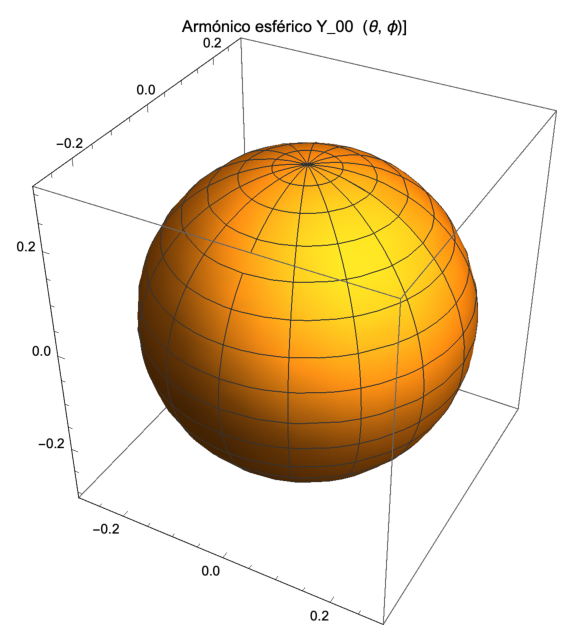
\includegraphics[scale=0.65]{Imagenes/Armonicos_Esfericos_00.eps}
\end{figure}
\end{frame}
\begin{frame}[plain]
\begin{figure}
    \centering
    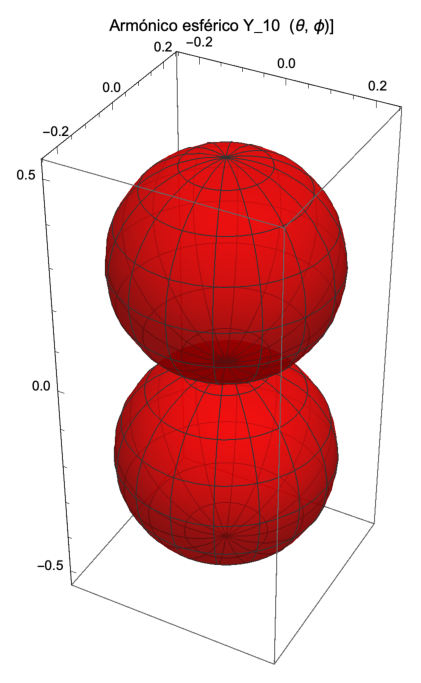
\includegraphics[scale=0.65]{Imagenes/Armonicos_Esfericos_10.eps}
\end{figure}
\end{frame}
\begin{frame}[plain]
\begin{figure}
    \centering
    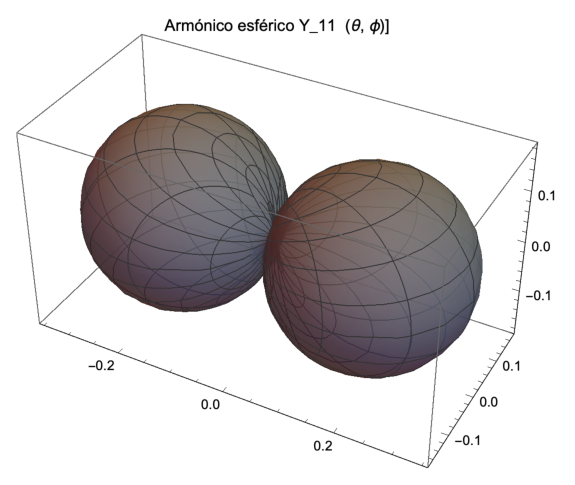
\includegraphics[scale=0.65]{Imagenes/Armonicos_Esfericos_11.eps}
\end{figure}
\end{frame}
\begin{frame}[plain]
\begin{figure}
    \centering
    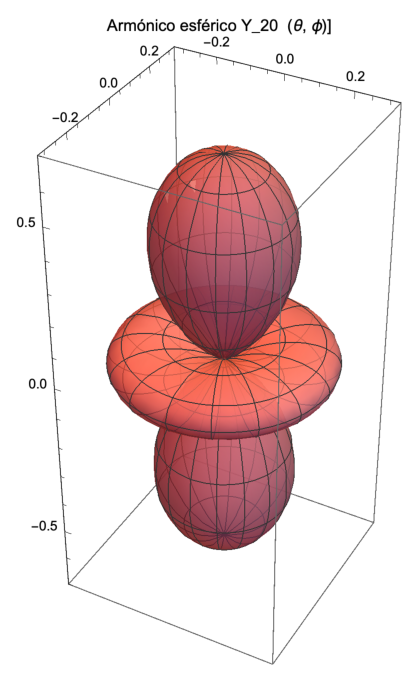
\includegraphics[scale=0.65]{Imagenes/Armonicos_Esfericos_20.eps}
\end{figure}
\end{frame}
\begin{frame}[plain]
\begin{figure}
    \centering
    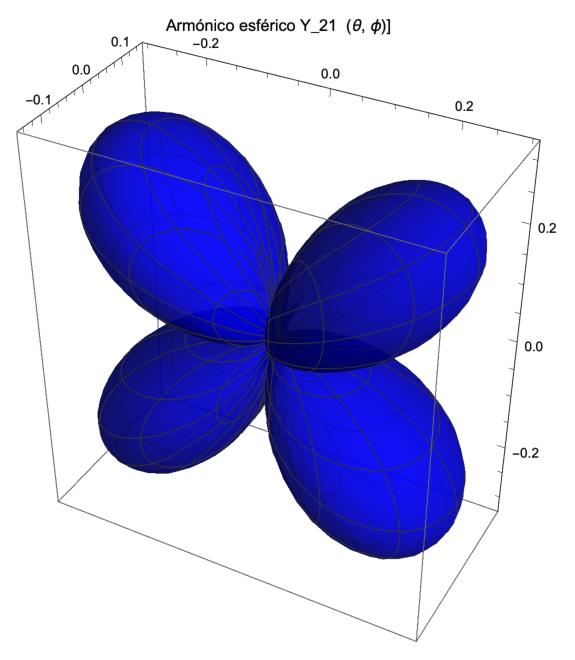
\includegraphics[scale=0.65]{Imagenes/Armonicos_Esfericos_21.eps}
\end{figure}
\end{frame}
\begin{frame}
\frametitle{Ortogonalidad de los armónicos esféricos}
Ya que contienen su $\theta$-dependiente de parte de la solución $P_{\ell}^{m}$ a la ecuación asociada de Legendre, \pause los $Y_{\ell}^{m}$ son mutuamente ortogonales cuando se integra de $-1$ a $+1$ sobre $d(cos \theta)$.
\end{frame}
\begin{frame}
\frametitle{Ortogonalidad de los armónicos esféricos}
Su ortogonalidad mutua respecto de $\phi (0 \leq \phi \leq 2 \pi)$ es aún más evidente. 
\\
\bigskip
\pause
El factor numérico en la ecuación (\ref{eq:ecuacion_045}) es elegido para hacer el $Y_{\ell}^{m}$ un conjunto ortonormal:
\end{frame}
\begin{frame}
\frametitle{Ortogonalidad de los armónicos esféricos}
Es decir:
\pause
\begin{equation}
\begin{aligned}[b]
\scaleint{6ex}_{-1}^{1} \scaleint{6ex}_{0}^{2 \pi} [ Y&_{\ell}^{m} (\theta, \phi) ]^{*} Y_{\ell'}^{m'} (\theta, \phi) d \phi d(\cos \theta) = \\[0.5em] 
&= \delta_{\ell \ell'} \delta_{m m'}
\end{aligned}
\label{eq:ecuacion_046}
\end{equation}
\end{frame}
\begin{frame}
\frametitle{Conjunto completo}
Adicionalmente, los armónicos esféricos forman un conjunto completo para cualquier función razonable de $\theta$ y $\phi$(como las que podemos encontrar en un problema físico).
\end{frame}
\begin{frame}
\frametitle{Conjunto completo}
La función puede expandirse como una suma de tales funciones:
\pause
\begin{equation}
f (\theta, \phi) = \nsum_{\ell=0}^{\infty} \nsum_{-\ell}^{\ell} a_{\ell m} \, Y_{\ell}^{m} (\theta, \phi)
\label{eq:ecuacion_047}
\end{equation}
\end{frame}
\begin{frame}
\frametitle{Conjunto completo}
Las constantes $a_{\ell m}$ están dadas por:
\pause
\begin{equation}
a_{\ell m} = \scaleint{6ex}_{-1}^{1} \scaleint{6ex}_{0}^{2 \pi} [ Y_{\ell}^{m} (\theta, \phi) ]^{*} f (\theta, \phi) \dd{\theta} \dd{(\cos \theta)}
\label{eq:ecuacion_048}
\end{equation}
\pause
Esto es una analogía exacta con una serie de Fourier y es un ejemplo particular de la propiedad general de soluciones de Sturm-Liouville.
\end{frame}

\subsection{Teorema de adición}

\begin{frame}
\frametitle{Teorema de adición}
Aparte de la condición ortonormalidad (\ref{eq:ecuacion_046}), \pause la relación más importante que cumplen los $Y_{\ell}^{m}$ es el teorema de adición de armónicos esféricos:
\pause
\begin{equation}
P_{\ell} (\cos \gamma) = \dfrac{4 \pi}{2 \ell + 1} \nsum_{m = -\ell}^{\ell} Y_{\ell}^{m} (\theta, \phi) [ Y_{\ell}^{m} (\pderivada{\theta}, \pderivada{\phi}) ]^{*}
\end{equation}
donde $(\theta, \phi)$ y $(\pderivada{\theta}, \pderivada{\phi})$ denotan dos direcciones diferentes a nuestro sistema de coordenadas esféricas polares y que están separadas por un ángulo $\gamma$.
\end{frame}
\begin{frame}
\frametitle{Teorema de adición}
En general, la trigonometría esférica (o vectorial) demuestra que estos ángulos obedecen la identidad:
\pause
\begin{equation}
\cos \gamma = \cos \theta \cos \pderivada{\theta} + \sin \theta \sin \pderivada{\theta} \cos (\phi - \pderivada{\phi})
\label{eq:ecuacion_050}
\end{equation}
\end{frame}

%Ref. Jackson 3.6 Problem Solution
\section{Ejercicio Teorema de Adición}
\frame{\tableofcontents[currentsection, hideothersubsections]}
\subsection{Enunciado}

\begin{frame}
\frametitle{Enunciado para el ejercicio}
Dos cargas puntuales $q$ y $-q$ se localizan sobre el eje $z$ en los puntos $z = +a$ y $z = -a$, respectivamente.
\pause
\begin{figure}[H]
    \centering
    \begin{tikzpicture}
        \draw (0, -2) -- (0, 2) node [right, pos=1] {$z$};
        \draw [fill] (0, 1) circle (0.1);
        \draw [fill] (0, -1) circle (0.1);
        \draw (-0.2, 0) -- (0.2, 0);
        \node at (0.5, 1) {$q$};
        \node at (0.5, -1) {$-q$};
        \node at (-0.5, 0.5) {$a$};
        \node at (-0.5, -0.5) {$-a$};
    \end{tikzpicture}
\end{figure}
\end{frame}
\begin{frame}
\frametitle{A resolver}
Por resolver:
\pause
\setbeamercolor{item projected}{bg=olive,fg=white}
\setbeamertemplate{enumerate items}{%
\usebeamercolor[bg]{item projected}%
\raisebox{1.5pt}{\colorbox{bg}{\color{fg}\footnotesize\insertenumlabel}}%
}
\begin{enumerate}[<+->]
\item \label{item:inciso_1} Calcula el potencial electrostático como una expansión de los armónicos esféricos y de potencias de $r$, tanto para $r > a$ y $r < a$.
\seti
\end{enumerate}
\end{frame}
\begin{frame}
\frametitle{A resolver}
\setbeamercolor{item projected}{bg=olive,fg=white}
\setbeamertemplate{enumerate items}{%
\usebeamercolor[bg]{item projected}%
\raisebox{1.5pt}{\colorbox{bg}{\color{fg}\footnotesize\insertenumlabel}}%
}
\begin{enumerate}[<+->]    
\conti
\item \label{item:inciso_2} Manteniendo el producto $q \, a = p /2$ constante, toma el límite cuando $a \to 0$ y calcula el potencial para $r \neq 0$. \pause Esto corresponde a la definición de un dipolo sobre el eje $z$ y su potencial.
\seti
\end{enumerate}
\end{frame}
\begin{frame}
\frametitle{A resolver}
\setbeamercolor{item projected}{bg=olive,fg=white}
\setbeamertemplate{enumerate items}{%
\usebeamercolor[bg]{item projected}%
\raisebox{1.5pt}{\colorbox{bg}{\color{fg}\footnotesize\insertenumlabel}}%
}
\begin{enumerate}[<+->]    
\conti
\item \label{item:inciso_3} Supongamos ahora que el dipolo del inciso \ref{item:inciso_2} está rodeado por una capa esférica de radio $b$ concéntrica en el origen, puesta a tierra. Por superposición lineal, encuentra el potencial en todas partes dentro del cascarón.
\end{enumerate}
\end{frame}

\subsection{Solución Inciso 1}

\begin{frame}
\frametitle{Usando la teoría de electromagnetismo}
\textbf{Inciso \ref{item:inciso_1}:} Usado la ley de Coulomb, podemos escribir de manera directa el potencial de dos cargas puntuales:
\pause
\begin{align*}
\Phi = \dfrac{q}{4 \pi \varepsilon_{0}} ~ \bigg[ \dfrac{1}{\abs{\vb{r} - a \, \vu{k}}} - \dfrac{1}{\abs{\vb{r} + a \, \vu{k}}} \bigg]
\end{align*}
\end{frame}
\begin{frame}
\frametitle{Usando la propiedad de completes}
Usando el teorema de adición, expandimos en factores de $1/R$:
\pause
\begin{align*}
\dfrac{1}{\abs{\vb{r} {-} \vb{\pderivada{r}}}} = 4 \pi \nsum_{\ell=0}^{\infty} \nsum_{m=-\ell}^{\ell} \dfrac{1}{2 \ell {+} 1} \, \dfrac{r_{<}^{\ell}}{r_{>}^{\ell+1}} \, Y_{\ell m}^{*} (\pderivada{\theta}, \pderivada{\phi}) \, Y_{\ell m} (\theta, \phi)
\end{align*}
\pause
donde:
\begin{align*}
r_{<} = \min \left\{ r, \pderivada{r} \right\} \hspace{1.5cm} r_{>} = \max \left\{ r, \pderivada{r} \right\}
\end{align*}
\end{frame}
\begin{frame}
\frametitle{Reescribiendo el potencial}
Entonces el potencial se escribe como:
\pause
\begin{align*}
&\Phi {=} \dfrac{q}{4 \pi \varepsilon_{0}} \bigg[ 4 \pi \nsum_{\ell=0}^{\infty} \nsum_{m=-\ell}^{\ell} \dfrac{1}{2 \ell {+} 1} \dfrac{r_{<}^{\ell}}{r_{>}^{\ell+1}} Y_{\ell m}^{*} (0, 0) Y_{\ell m} (\theta, \phi) + \\[0.5em]
&- 4 \pi \nsum_{\ell=0}^{\infty} \nsum_{m=-\ell}^{\ell} \dfrac{1}{2 \ell {+} 1} \, \dfrac{r_{<}^{\ell}}{r_{>}^{\ell+1}} \, Y_{\ell m}^{*} (\pi, 0) \, Y_{\ell m} (\theta, \phi) \bigg]
\end{align*}
\pause
Ahora se tiene que:
\pause
\begin{align*}
r_{<} = \min \left\{ r, a \right\} \hspace{1.5cm} r_{>} = \max \left\{ r, a \right\}
\end{align*}
\end{frame}
\begin{frame}
\frametitle{Reorganizando la expresión}
Cancelando el término $4 \pi$ y factorizando las sumas con el armónico $Y_{\ell m} (\theta, \phi)$, el potencial queda:
\pause
\begin{align*}
\Phi &= \dfrac{q}{\varepsilon_{0}} ~ \nsum_{\ell=0}^{\infty} \nsum_{m=-\ell}^{\ell} \dfrac{1}{2 \ell + 1} \, \dfrac{r_{<}^{\ell}}{r_{>}^{\ell+1}} \, \times \\[0.5em]
&\times Y_{\ell m} (\theta, \phi) \bigg[ Y_{\ell m}^{*} (0, 0) - Y_{\ell m}^{*} (\pi, 0) \bigg]    
\end{align*} 
\end{frame}
\begin{frame}
\frametitle{Expresión para $r < a$}
Haciendo de manera explícita cada caso para $r$, se tiene que:
\pause
\begin{align*}
\Phi &= \dfrac{q}{\varepsilon_{0}} \,\nsum_{\ell=0}^{\infty} \nsum_{m=-\ell}^{\ell} \dfrac{1}{2 \ell {+} 1} \dfrac{r_{\ell}}{a^{\ell+1}} \, \times \\[0.5em]
&\times Y_{\ell m} (\theta, \phi) \bigg[ Y_{\ell m}^{*} (0, 0) {-} Y_{\ell m}^{*} (\pi, 0) \bigg]
\end{align*}
\end{frame}
\begin{frame}
\frametitle{Expresión para $r > a$}
\begin{align*}
\Phi &= \dfrac{q}{\varepsilon_{0}} \nsum_{\ell=0}^{\infty} \nsum_{m=-\ell}^{\ell} \dfrac{1}{2 \ell {+} 1} \dfrac{a^{\ell}}{r^{\ell+1}} \, \times \\[0.5em]
&\times Y_{\ell m} (\theta, \phi) \bigg[ Y_{\ell m}^{*} (0, 0) {-} Y_{\ell m}^{*} (\pi, 0) \bigg]
\end{align*}
\end{frame}
\begin{frame}
\frametitle{Misión cumplida}
La pregunta original pedía la respuesta en términos de los armónicos esféricos, así que eso es lo que hemos dado.
\\
\bigskip
\pause
Sin embargo, podemos simplificar la respuesta.
\end{frame}
\begin{frame}
\frametitle{Aprovechando la simetría}
Tengamos en cuenta que el problema presenta simetría azimutal, \pause por lo que la solución debe ser azimutalmente simétrica.
\\
\bigskip
\pause
Esto significa que todos los términos de la serie excepto el término $m = 0$ deben anularse:
\end{frame}
\begin{frame}
\frametitle{Consecuencia de la simetría}
\begin{eqnarray*}
\begin{aligned}
\Phi &= \pause \dfrac{q}{\varepsilon_{0}} \nsum_{\ell=0}^{\infty}  \dfrac{1}{2 \ell {+} 1} \dfrac{r_{<}^{\ell}}{r_{>}^{\ell+1}} Y_{\ell 0} (\theta, \phi) \bigg[ Y_{\ell 0}^{*} (0, 0) {-} Y_{\ell 0}^{*} (\pi, 0) \bigg] = \\[0.5em] \pause
&= \dfrac{q}{4 \pi \varepsilon_{0}} \nsum_{\ell=0}^{\infty} \dfrac{r_{<}^{\ell}}{r_{>}^{\ell+1}} \, P_{\ell} (\cos \theta) \bigg[ P_{\ell} (1) - P_{\ell} (-1) \bigg] = \\[0.5em] \pause
&= \dfrac{q}{4 \pi \varepsilon_{0}} \nsum_{\ell=0}^{\infty} \dfrac{r_{<}^{\ell}}{r_{>}^{\ell+1}} \, P_{\ell} (\cos \theta) \bigg[ 1 - (-1)^{\ell} \bigg]
\end{aligned}
\end{eqnarray*}
\end{frame}
\begin{frame}
\frametitle{Potencial electróstatico}
Por lo que el potencial electrostático está dado por:
\pause
\begin{align*}
\Phi = \dfrac{2 q}{4 \pi \varepsilon_{0}} \nsum_{\ell=0, \text{impar}}^{\infty} \dfrac{r_{<}^{\ell}}{r_{>}^{\ell+1}} \, P_{\ell} (\cos \theta)
\end{align*}
donde:
\pause
\begin{align*}
r_{<} = \min \left\{ r, a \right\} \hspace{1.5cm} r_{>} = \max \left\{ r, a \right\}
\end{align*}
\end{frame}

\subsection{Solución Inciso 2}

\begin{frame}
\frametitle{El inciso 2}
Manteniendo el producto $q \, a = p /2$ constante, toma el límite cuando $a \to 0$ y calcula el potencial para $r \neq 0$.
\\
\bigskip
\pause
Con esta condición, siempre estaremos en la región $r > a$. 
\end{frame}
\begin{frame}
\frametitle{Usando el resultado del inciso 1}
Del resultado del inciso \ref{item:inciso_1}, se tiene que:
\pause
\begin{align*}
\Phi = \dfrac{2 q}{4 \pi \varepsilon_{0}} \nsum_{\ell=0, \text{impar}}^{\infty} \dfrac{a^{\ell}}{r^{\ell+1}} \, P_{\ell} (\cos \theta)
\end{align*}
\end{frame}
\begin{frame}
\frametitle{Condición del enunciado}
Como $p = 2 q a$, resulta:
\pause
\begin{eqnarray*}
\begin{aligned}
\Phi &= \dfrac{p}{4 \pi \varepsilon_{0}} \nsum_{\ell=0, \text{impar}}^{\infty} \dfrac{a^{\ell-1}}{r^{\ell+1}} \, P_{\ell} (\cos \theta) = \\[0.5em] \pause
&= \dfrac{p}{4 \pi \varepsilon_{0}} \bigg[ \dfrac{1}{r^{2}} P_{1} (\cos \theta) {+} \dfrac{a^{2}}{r^{4}} P_{3} (\cos \theta) + \\[0.5em]
&+ \dfrac{a^{4}}{r^{6}} P_{5} (\cos \theta) {+} \ldots \bigg]
\end{aligned}
\end{eqnarray*}
\end{frame}
\begin{frame}
\frametitle{Caso con el límite}
Cuando $a \to 0$, se obtiene:
\pause
\begin{align*}
\setlength{\fboxsep}{3\fboxsep}\boxed{
\Phi = \dfrac{p}{4 \pi \varepsilon_{0}} \, \dfrac{1}{r^{2}} \, \cos \theta }
\end{align*}
\pause
Este es el potencial de un dipolo perfecto en el origen que apunta a lo largo del eje $z$.
\end{frame}
\subsection{Solución Inciso 3}


\begin{frame}
\frametitle{Enunciado del Inciso 3}
\textbf{Inciso \ref{item:inciso_3}: } Si el dipolo del inciso \ref{item:inciso_2} está rodeado por una capa esférica conectada a tierra de radio $b$ concéntrica con el origen:
\setbeamercolor{item projected}{bg=olive,fg=white}
\setbeamertemplate{enumerate items}{%
\usebeamercolor[bg]{item projected}%
\raisebox{1.5pt}{\colorbox{bg}{\color{fg}\footnotesize\insertenumlabel}}%
}
\begin{enumerate}[<+->]
\item Habrá un potencial adicional debido a la esfera.
\item El potencial total en la superficie debe ser cero.
\end{enumerate}
\end{frame}
\begin{frame}
\frametitle{Ocupando el resultado del inciso 2}
Del resultado del inciso \ref{item:inciso_2}:
\pause
\begin{align*}
\Phi = \dfrac{p}{4 \pi \varepsilon_{0}} \, \dfrac{1}{r^{2}} \, \cos \theta
\end{align*}
\end{frame}
\begin{frame}
\frametitle{Sumando el otro potencial}
Agregamos el potencial adicional:
\pause
\begin{align*}
\Phi = \dfrac{p}{4 \pi \varepsilon_{0}} \, \dfrac{1}{r^{2}} \, \cos \theta + \nsum_{\ell=0}^{\infty} A_{\ell} \, r^{\ell} \, P_{\ell} (\cos \theta)
\end{align*}
\end{frame}
\begin{frame}
\frametitle{Usando la CDF}
Aplicando la condición de frontera:
\pause
\begin{eqnarray*}
\begin{aligned}
0 &= \dfrac{p}{4 \pi \varepsilon_{0}} \, \dfrac{1}{r^{2}} \, \cos \theta + \nsum_{\ell=0}^{\infty} A_{\ell} \, b^{\ell} \, P_{\ell} (\cos \theta) \\[0.5em] \pause
\Rightarrow \hspace{0.2cm} &- \dfrac{p}{4 \pi \varepsilon_{0}} \, \dfrac{1}{b^{2}} \, \cos \theta = \nsum_{\ell=0}^{\infty} A_{\ell} \, b^{\ell} \, P_{\ell} (\cos \theta)
\end{aligned}
\end{eqnarray*}
\end{frame}
\begin{frame}
\frametitle{Usando propiedades de los $P_{\ell} (\cos \theta)$}
Debido a la condición de ortogonalidad, solo el término $\ell = 1$ es no nulo:
\pause
\begin{align*}
A_{1} = - \dfrac{p}{4 \pi \varepsilon_{0}} \, \dfrac{1}{b^{3}}
\end{align*}
\end{frame}
\begin{frame}
\frametitle{Potencial en puntos internos}
Entonces el potencial en puntos dentro del cascarón está dado por:
\pause
\begin{align*}
\setlength{\fboxsep}{3\fboxsep}\boxed{
\Phi = \dfrac{p \, \cos \theta}{4 \pi \varepsilon_{0}} ~ \bigg[ \bigg( \dfrac{b}{r} \bigg)^{2} - \dfrac{r}{b} \bigg] \qed}
\end{align*}
\end{frame}

\end{document}